% This file was created with tikzplotlib v0.10.1.
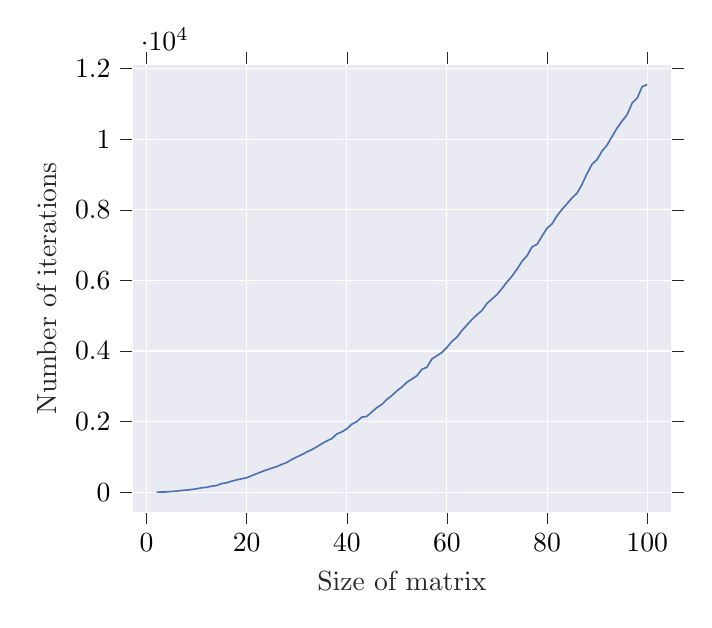
\begin{tikzpicture}

\definecolor{darkslategray38}{RGB}{38,38,38}
\definecolor{lavender234234242}{RGB}{234,234,242}
\definecolor{steelblue76114176}{RGB}{76,114,176}

\begin{axis}[
axis background/.style={fill=lavender234234242},
axis line style={white},
mark options={mark size=2.5pt, line width=1.5pt},
minor xtick={},
minor ytick={},
tick align=outside,
title style={align=center},
x grid style={white},
xlabel=\textcolor{darkslategray38}{Size of matrix},
xmajorgrids,
xmajorticks=false,
xmajorticks=true,
xmin=-2.9, xmax=104.9,
xtick style={color=darkslategray38},
xtick={-20,0,20,40,60,80,100,120},
y grid style={white},
ylabel=\textcolor{darkslategray38}{Number of iterations},
ymajorgrids,
ymajorticks=false,
ymajorticks=true,
ymin=-576.45, ymax=12127.45,
ytick style={color=darkslategray38},
ytick={-2000,0,2000,4000,6000,8000,10000,12000,14000}
]
\addplot [semithick, steelblue76114176]
table {%
2 1
3 4
4 8
5 20
6 28
7 49
8 61
9 77
10 94
11 125
12 138
13 170
14 190
15 243
16 267
17 312
18 349
19 380
20 409
21 468
23 581
24 633
25 680
26 725
27 788
28 839
29 927
30 997
31 1063
32 1139
33 1204
34 1286
35 1372
36 1452
37 1519
38 1650
39 1709
40 1796
41 1927
42 2002
43 2127
44 2147
45 2276
46 2396
47 2489
48 2631
49 2736
50 2871
51 2979
52 3114
54 3300
55 3481
56 3541
57 3775
58 3866
59 3960
60 4102
61 4274
62 4392
63 4581
65 4894
66 5030
67 5149
68 5349
70 5600
71 5772
72 5957
73 6122
74 6319
75 6544
76 6700
77 6950
78 7022
79 7256
80 7481
81 7603
82 7835
83 8015
84 8175
85 8341
86 8475
87 8727
88 9031
89 9297
90 9426
91 9671
92 9837
93 10083
94 10321
95 10518
96 10701
97 11025
98 11166
99 11491
100 11550
};
\end{axis}

\end{tikzpicture}
